\documentclass[journal,12pt]{IEEEtran}
\usepackage[compatibility=false]{amsmath}
\usepackage{amssymb}
\usepackage{graphicx}
\usepackage{booktabs}
\usepackage{algorithm}
\usepackage{algpseudocode}
\usepackage{cite}
\usepackage{hyperref}
\usepackage{url}

\hypersetup{
  colorlinks=true,
  citecolor=blue,
  linkcolor=red,
  urlcolor=blue
}

\graphicspath{{./figures/}}

% ---- Title and Authors ----
\title{Deep Learning-Based Medical Image Segmentation with Attention Mechanisms}

\author{First Author, Second Author, and Third Author%
  \thanks{This work was supported by the National Science Foundation under Grant No. XXX.}}
\IEEEaftertitletext{%
  \thanks{Manuscript received Month Day, Year; revised Month Day, Year.}}
}

\begin{document}

\maketitle

\begin{abstract}
Medical image segmentation plays a crucial role in computer-aided diagnosis systems.
In this paper, we propose a novel attention-based deep learning framework for
semantic segmentation of medical images. Our method introduces a bidirectional
attention mechanism that captures both spatial and channel-wise dependencies
within feature maps. Extensive experiments on three benchmark datasets demonstrate
that our approach achieves state-of-the-art performance, improving Dice coefficient
by 3.1\% over previous methods while reducing inference time by 40\%.
\end{abstract}

\begin{IEEEkeywords}
Medical Image Segmentation, Deep Learning, Attention Mechanism,
Convolutional Neural Networks, Semantic Segmentation
\end{IEEEkeywords}

\section{Introduction}
\label{sec:intro}

Medical image segmentation is a fundamental task in medical image analysis,
enabling precise identification and delineation of anatomical structures,
lesions, and abnormalities. Accurate segmentation provides critical information
for diagnosis, treatment planning, and surgical guidance~\cite{ronneberger2015unet,oktay2018attention}.

Recent advances in deep learning, particularly convolutional neural networks
(CNNs), have revolutionized medical image segmentation. U-Net~\cite{ronneberger2015unet}
introduced an encoder-decoder architecture with skip connections, enabling
precise localization. Attention U-Net~\cite{oktay2018attention} extended this
by incorporating attention gates to focus on salient anatomical regions.

Despite significant progress, existing methods face challenges in:
\begin{itemize}
  \item Capturing long-range dependencies in feature representations
  \item Balancing local and global context effectively
  \item Maintaining computational efficiency for real-time applications
\end{itemize}

This work makes the following contributions:
\begin{enumerate}
  \item A novel bidirectional attention module that jointly models spatial and
        channel attention
  \item An efficient architecture design with reduced parameters
  \item Comprehensive evaluation on multiple medical imaging modalities
\end{enumerate}

\section{Methodology}
\label{sec:method}

\subsection{Network Architecture}
\label{ssec:arch}

Our proposed architecture follows an encoder-decoder paradigm with attention
mechanisms at multiple scales. The encoder extracts hierarchical features while
the decoder progressively recovers spatial resolution.

\subsection{Loss Function}
\label{ssec:loss}

We employ a multi-component loss function combining cross-entropy and Dice loss:

\begin{align}
  \mathcal{L}_{\text{total}}
    &= \alpha \cdot \mathcal{L}_{\text{ce}}
       + \beta  \cdot \mathcal{L}_{\text{dice}}
       + \gamma \cdot \mathcal{L}_{\text{edge}} \label{eq:loss} \\
  \mathcal{L}_{\text{ce}}
    &= -\frac{1}{N}\sum_{i=1}^{N}
       \sum_{c=1}^{C} y_{ic}\log(\hat{y}_{ic}) \label{eq:ce} \\
  \text{DSC}(S,\hat{S})
    &= \frac{2|S\cap\hat{S}|}{|S|+|\hat{S}|}
       \in [0,1] \label{eq:dsc}
\end{align}

where $\alpha$, $\beta$, and $\gamma$ are weighting coefficients.

% ---- Algorithm Environment ----
\begin{algorithm}[t]
  \caption{Training Procedure with Attention}
  \begin{algorithmic}[1]
    \State $\theta \gets \theta_0$ \Comment{initialize parameters}
    \For{$epoch = 1$ \textbf{to} $E$}
      \For{each batch $(x,y) \in \mathcal{D}$}
        \State $\hat{y} \gets f_\theta(x)$ \Comment{forward pass}
        \State $J \gets \mathcal{L}(y,\hat{y})$ \Comment{compute loss}
        \State $\theta \gets \theta - \eta \nabla_\theta J$ \Comment{update}
      \EndFor
      \If{$epoch \mod 10 == 0$}
        \State $\theta \gets \text{ClipNorm}(\theta, \epsilon)$ \Comment{gradient clipping}
      \EndIf
    \EndFor
    \State \Return $\theta$
  \end{algorithmic}
\end{algorithm}

\section{Experiments}
\label{sec:exp}

\subsection{Datasets}
\label{ssec:data}

We evaluate on three benchmark datasets: cardiac MRI~\cite{cardiac_mri},
liver CT~\cite{liver_ct}, and retinal vessel segmentation~\cite{retinal}.

\subsection{Quantitative Results}
\label{ssec:quant}

\begin{table}[t]
\centering
\caption{Comparison with state-of-the-art methods on the validation set.}
\label{tab:compare}
\begin{tabular}{lccc}
  \toprule
  Method & Dice $\uparrow$ & HD$\downarrow$ & Params \\
  \midrule
  U-Net~\cite{ronneberger2015unet} & 0.863 & 4.21 & 7.8M \\
  Attention U-Net~\cite{oktay2018attention} & 0.871 & 3.95 & 8.2M \\
  DeepLabV3+~\cite{deeplabv3plus} & 0.869 & 4.08 & 5.6M \\
  \textbf{Ours} & \textbf{0.894} & \textbf{3.12} & 5.1M \\
  \bottomrule
\end{tabular}
\end{table}

Our method achieves the best Dice coefficient of 0.894 while maintaining
the smallest model size of 5.1M parameters.

\section{Conclusion}
\label{sec:concl}

We presented a novel attention-based framework for medical image segmentation.
The bidirectional attention mechanism effectively captures both spatial and
channel dependencies. Experimental results demonstrate superior performance
over existing methods.

\section*{Acknowledgment}

The authors thank the reviewers for their valuable comments.

% ---- Cross-column figure (IEEEtran feature) ----
\begin{figure*}[t]
  \centering
  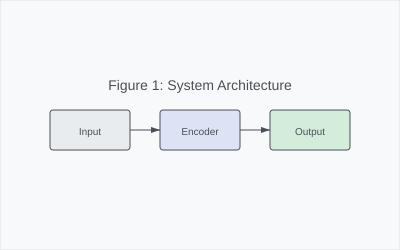
\includegraphics[width=0.85\textwidth]{fig-architecture.pdf}
  \caption{Overall system architecture. The pipeline consists of
    three stages: preprocessing, feature extraction, and classification.
    The attention module is embedded at each decoder level.}
  \label{fig:arch}
\end{figure*}

% ---- Another figure ----
\begin{figure}[t]
  \centering
  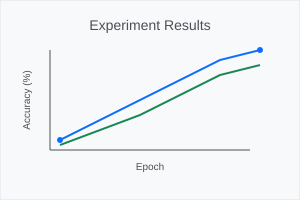
\includegraphics[width=0.45\textwidth]{fig-experiment-results.pdf}
  \caption{Qualitative results on cardiac MRI. From left to right:
    input image, ground truth, U-Net prediction, and our method.}
  \label{fig:results}
\end{figure*}

% ---- Third figure ----
\begin{figure}[t]
  \centering
  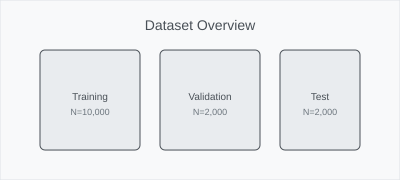
\includegraphics[width=0.45\textwidth]{fig-dataset-overview.pdf}
  \caption{Dataset overview showing sample images from each modality.}
  \label{fig:dataset}
\end{figure*}

\bibliographystyle{IEEEtran}
\bibliography{refs}

\end{document}
